\begin{figure}
  \centering
  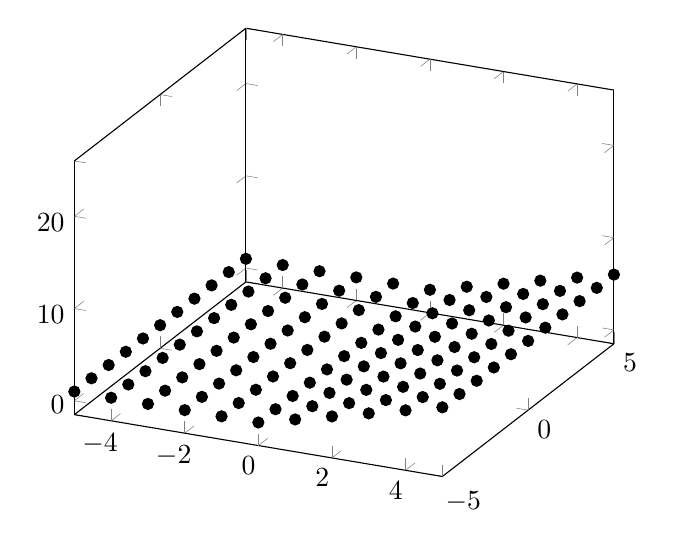
\begin{tikzpicture}
    \begin{axis}[zmax=26]
      \addplot3 [
        unbounded coords=jump,
        mesh,
        shader=interp,
        samples at={-5,...,5},
        samples y={11},
        only marks,
      ] {1+max(x,0)};
    \end{axis}
  \end{tikzpicture}
  \hfil
  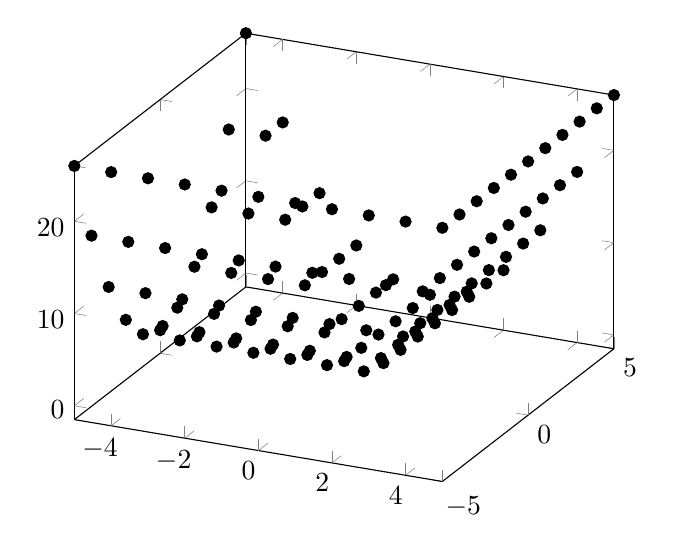
\begin{tikzpicture}
    \begin{axis}[zmax=26]
      \addplot3 [
        unbounded coords=jump,
        mesh,
        shader=interp,
        samples at={-5,...,5},
        samples y={11},
        only marks,
      ] {1+abs(max(x,-y))*abs(max(x,-y))};
    \end{axis}
  \end{tikzpicture}
  \caption{Evaluation of an example where cost ranking functions yield a benefit}
  \label{fig:cost_ranking_function}
\end{figure}
